\chapter{Engineering Research Problem}
\setcounter{page}{1}
\label{chap:chap1}

\section{Background }
As the use of Artificial Intelligence (AI) and Machine 
Learning (ML) continues to grow throughout the world 
in high-risk applications, models have become 
ever-increasingly complex and diverse. As a result, 
they often become prone to accidents where unintended 
and harmful behaviour is observed, and consequently are 
scrutinized as disruptive and unreliable solutions. The 
recent emergence in smart cities have seen AI and ML being 
used in various applications such as transportation, 
healthcare, environmental, and public safety as depicted in Figure (\ref{fig:smart}).

\begin{figure}[h]
    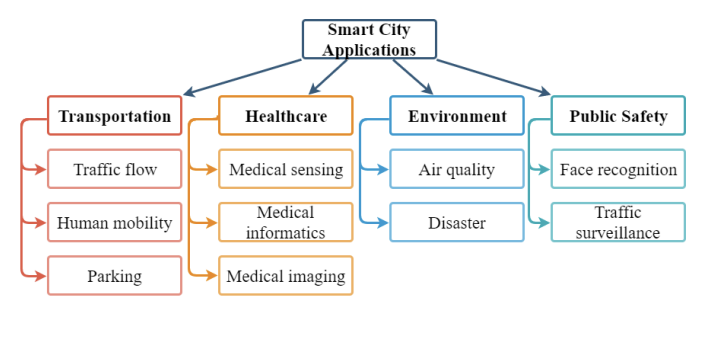
\includegraphics{smart_city_applications.png}
    \caption{Smart City Artificial Intelligence Applications \cite{chen}}
    \label{fig:smart}
\end{figure}

\enlargethispage{2\baselineskip}
For an AI/ML system to be considered reliable, it must 
perform tasks when required as it was originally 
intended, produce consistent results using real-world 
data (and shifts in data), and remain robust and 
predictable. This means it must also fail in a 
predictable manner \cite{Saif}. 

\section{Applications}
One of the most discussed and disruptive applications of ML is facial 
recognition systems used by authorities which fails to distinguish 
between darker skin individuals. This technology is used to assist the 
police in identifying potential criminals/suspects and often leads to 
wrongful arrests of dark-skinned people \cite{Moutafis}. This example highlights the 
importance and the need for reliability in ML solutions. 

There are many more applications where reliability is crucial due to the 
potential consequences. For example, cancer diagnosis systems trialled in the US fail to detect 
cancer in patients in differing hospitals and/or countries, resulting in death.
 As another example, unintended behaviours in traffic management systems would 
increase congestion resulting in poor ambient air quality and noise 
pollution.

The rapid technological changes in manufacturing have produced a boom 
in Industry 4.0 applications involving Artificial Intelligence, connected
 devices (IoT) and Big Data. A paper on use cases of AI in Industry 4.0 
 summarises the advantages ML, \textit{“AI with machine learning technique can 
 automate the manufacturing process which increase the productivity, 
 efficiency, optimize production cost and reduce manual error” }\cite{9004327}. A 
 key area is predictive maintenance, where real-time equipment data is 
 captured and historical equipment data is evaluated using AI and ML 
 models to estimate the equipment life cycle and hence perform timely 
 maintenance to reduce or eliminate down-time. Downtime is undesirable
for manufacturers as it equates to the loss of revenue.

AI in cybersecurity helps protect enterprises by detecting unusual 
activity, patterns, and malicious behaviour and can respond to different 
situations. For manufacturers, this could be used for asset protection 
while banks and financial institutions may use this form ML to detect suspicious 
activity and fraud \cite{9004327}. 

\section{Project Contextualisation}
A tutorial presented by Suchi Saria and Adarsh Subbaswamy of John Hopkins University \cite{saria2019tutorial} postulates some causes and failure prevention techniques for use in supervised learning systems (regression and classification). 
Some of the sources of unreliability discussed in this tutorial are inadequate data, changes in training and deployment environments, and model misspecification. 
These causes mentioned above will form the basis of this research project.

\enlargethispage{-\baselineskip}
Another reliability issue is discussed in a separate paper, \textit{‘Concrete Problems in AI Safety’} \cite{Amodei}, is the prevalence of reward hacking in Reinforcement Learning systems. 
\textit{Reward hacking} is defined as the AI agent’s ability to cheat the system to achieve the highest reward in an unintended way. 
For example, a positive reward may be given to a traffic management system when there is no congestion. However, the AI model decides to divert all traffic through alternative routes, essentially shutting down this particular road/intersection. 
This prevents congestion but does not perform as desired. This notion is also investigated in this research project.

In Chapter \ref{chap:chap2,} we outline the methodologies used throughout this report.
Chapter \ref{chap:chap3} discusses how bias arises in datasets through labelling and datashift.
Experimentation is performed to show that bias exists before solutions for reducing bias are described.
Chapter \ref{chap:chap4} examines the factors which impact algorithm selection on a number of Artificial Intelligence applications.
Subsequently, methods to improve the reliability and performance of algorithms are discussed.
Afterwards, in Chapter \ref{chap:chap5}, the causes and prevention approaches of reward hacking in RL systems are discussed.

\section{Research Question}
\noindent\rule{\linewidth}{0.4pt}
\begin{quotation}
\textit{How can the reliability of Artificial Intelligence be improved against 
inadequate data labelling, unsuitable algorithm choices, and reward 
hacking?}
\end{quotation}
\noindent\rule{\linewidth}{0.4pt}